\documentclass[a4paper]{article}
\usepackage{amsmath}
\usepackage{graphicx}

\usepackage[a4paper, margin=3cm]{geometry}

\usepackage[T1]{fontenc}
\usepackage[utf8]{inputenc}
\usepackage[serbian]{babel}
\usepackage{subfigure}	% needed for inserting figures
\usepackage{hyperref}
\usepackage{amsmath}
\usepackage{amssymb}
\usepackage[justification=centering]{caption}

\usepackage{hyperref}
\hypersetup{
    colorlinks=true,
    linkcolor=blue,
    filecolor=magenta,      
    urlcolor=cyan,
}

\begin{document}
\newcommand{\mr}[1]{\mathrm{#1}}
\renewcommand{\figurename}{Slika}
\pagenumbering{gobble}

\begin{center}
\huge{\textbf{\textsc{Hardversko softverska \\obrada signala\\Projekat za 2022/23. godinu}}}
\end{center}


\begin{center}
\large{\textbf{\textsc{Opis problema}}}
\end{center}

Na slici je prikazan blok dijagram programabilnog generatora signala.
Ulaz u generator signala je kompleksni signal u osnovnom opsegu učestanosti $x=I+\mr{j} Q$ učestanosti odabiranja 61.44~MHz. Spektar kompleksnog signala u osnovnom opsegu učestanosti \textbf{nije} konjugovano-kompleksno simetričan i koristan signal zauzima opseg učestanosti od -25 do +25 MHz. 
Odbirci test signala su dati u fajlu \texttt{python/testsignal.txt}.

\begin{center}
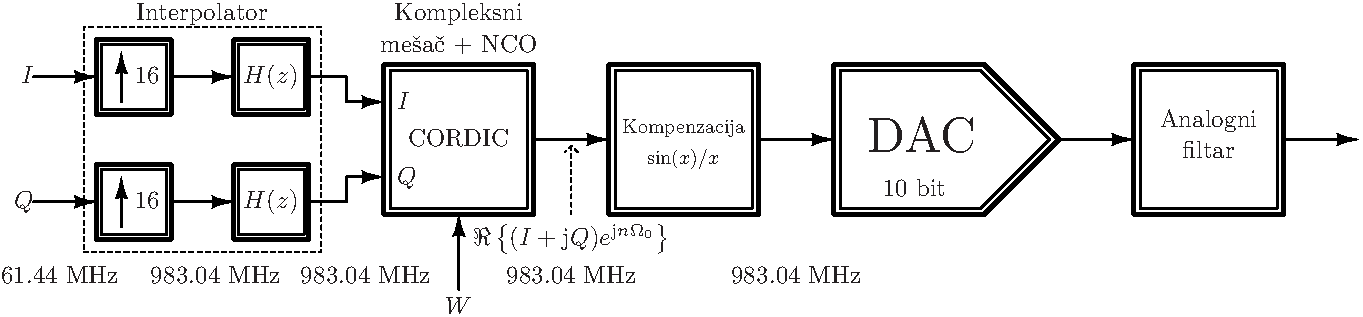
\includegraphics[width=\textwidth]{fig/block_diagram.pdf}
\end{center}

Učestanost odabiranja ulaznog signala se povećava $M=16$ puta interpolatorom. 
Interpolirani signal se zatim pomera na zadatu centralnu digitalnu učestanost $\Omega_0$ kompleksnim mešačem sa numerički kontrolisanim oscilatorom, što je ekvivalentno množenju odbiraka interpoliranog signala $x_I[n]$ kompleksnom sinusoidom $e^{\mr{j}\Omega_0 n}$ i uzimanjem realnog dela rezultata.
Na izlazu kompleksnog mešača se nalazi FIR filtar za kompenzaciju frekvencijskog odziva kola za rekonstrukciju digitalno-analognog konvertora.
Digitalno-analogni konvertor može raditi u NRZ ili RF modu, kako bi se omogućila rekonstrukcija signala u prvoj ili drugoj Nikvistovoj zoni.

\begin{center}
\large{\textbf{\textsc{Prva faza projekta}}}
\end{center}

U prvoj fazi projekta je potrebno uraditi:

\begin{enumerate}
\item $[10]$ Predložiti arhitekturu interpolatora sa odnosom promene učestanosti odabiranja od 16 puta. Nacrtati spektar signala, granične učestanosti filtara i učestanosti odabiranja u svim granama predložene arhitekture.
Pod pretpostavkom da je potrebno obezbediti potiskivanje spektralnih replika od $A_\mr{dB}=60~\mr{dB}$, proceniti ukupan broj računskih operacija u sekundi predložene arhitekture interpolatora i uporediti sa direktnom implementacijom.
\item $[10]$ Nacrtati blok dijagram realizacije kompleksnog mešača i numerički kontrolisanog oscilatora (NCO) primenom CORDIC algoritma. Predložiti minimalni broj iteracija CORDIC algoritma, širinu binarnih reči i broja zaštitnih bita. Odrediti minimalnu širinu kontrolne reči $W$ kojom se obezbeđuje frekvencijska rezolucija od 1~Hz.
\item $[5]$ Odrediti koeficijente FIR filtra za kompenzaciju frekvencijskog odziva NRZ kola za rekonstrukciju signala, tako da se amplituda rekonstruisanog signala ne menja više od $\pm 0.025~\mr{dB}$ u opsegu digitalnih učestanosti $F=[0,0.4]$.
\item $[5]$ Odrediti maksimalno vreme podrhtavanja trenutka odabiranja $t_\mr{j}$ tako da su na učestanosti $f=0.9 M f_\mr{s}=884.74~\mr{MHz}$ odnosi signal/šum usled kvantizacije i podrhtavanja izjednačeni.


\end{enumerate}

\begin{center}
\large{\textbf{\textsc{Druga faza projekta - hardverska realizacija}}}
\end{center}

\begin{enumerate}
\item $[20]$ U izabranom jeziku za opis hardvera implementirati protočnu realizaciju CORDIC algoritma sa parametrima određenim u prvoj fazi projekta.
\item $[20]$ Simulirati rad projektovanog CORDIC jezgra u modu kompleksnog mešača koji pomera ulazni signal na centralnu učestanost od 196.16~MHz. Nacrtati spektre ulaznog i izlaznog signala.
\end{enumerate}

\begin{center}
\large{\textbf{\textsc{Druga faza projekta - softverska realizacija}}}
\end{center}

\begin{enumerate}
\item $[10]$ Odrediti koeficijente filtara u interpolatoru. Prodiskutovati detalje implementacije filtara - polifaznu dekompoziciju, postupak izračunavanja izlaznih odbiraka. Nacrtati amplitudske karakteristike pojedinačnih filtara i ukupnu frekvencijsku karakteristiku.
\item $[10]$ Napraviti model CORDIC kompleksnog mešača u izabranom softverskom okruženju (Python, Octave, Matlab...). Simulirati rad CORDIC algoritma sa konstantnim ulaznim signalom i nacrtati spektar izlaznog signala. Izabrati učestanost izlaznog signala i broj odbiraka tako da budu zadovoljeni uslovi koherentnog odabiranja.
\item $[10]$ Napraviti model celog sistema u izabranom softverskom okruženju (Python, Octave, Matlab...).
\item $[10]$ Simulirati rad projektovanog sistema sa NRZ kolom za rekonstrukciju koji pomera ulazni signal na centralnu učestanost od $3M f_\mr{s}/8=368.64$~MHz. Nacrtati spektre ulaznog i izlaznog signala. Ponoviti simulaciju sa RF kolom za rekonstrukciju \textbf{u drugoj Nikvistovoj zoni} na centralnoj učestanosti od 860.16~MHz.
\end{enumerate}

\begin{center}
\large{\textbf{\textsc{Napomene}}}
\end{center}

\begin{itemize}

	\item Primeri Python skripti za crtanje amplitudskog odziva filtara i projektovanje poluopsežnih  filtara su dati u direktorijumu \texttt{python}.

	\item Spektar signala se može nacrtati i bez primene prozorske funkcije ukoliko se izvrši periodično produženje signala u trajanju kašnjenja interpolacionog filtra. Pogledati primer u Jupyter svesci.

	\item Izveštaji o prvoj i drugoj fazi projekta se pišu u formi rada za časopis u 
\href{https://journals.ieeeauthorcenter.ieee.org/create-your-ieee-journal-article/authoring-tools-and-templates/ieee-article-templates/templates-for-transactions}{MS Word ili \LaTeX~obrascu}
za IEEE Transactions on Microwave Theory and Techniques.

	\item Blok dijagrami se mogu nacrtati u programskom paketu 
		\href{http://opencircuitdesign.com/xcircuit/}{XCircuit}  uz pomoć 
		biblioteke simbola dsp.lps.

	\item Izveštaji se predaju isključivo u PDF formatu.
\end{itemize}

\end{document}
